% THIS IS SIGPROC-SP.TEX - VERSION 3.1
% WORKS WITH V3.2SP OF ACM_PROC_ARTICLE-SP.CLS
% APRIL 2009
%
% It is an example file showing how to use the 'acm_proc_article-sp.cls' V3.2SP
% LaTeX2e document class file for Conference Proceedings submissions.
% ----------------------------------------------------------------------------------------------------------------
% This .tex file (and associated .cls V3.2SP) *DOES NOT* produce:
%       1) The Permission Statement
%       2) The Conference (location) Info information
%       3) The Copyright Line with ACM data
%       4) Page numbering
% ---------------------------------------------------------------------------------------------------------------
% It is an example which *does* use the .bib file (from which the .bbl file
% is produced).
% REMEMBER HOWEVER: After having produced the .bbl file,
% and prior to final submission,
% you need to 'insert'  your .bbl file into your source .tex file so as to provide
% ONE 'self-contained' source file.
%
% Questions regarding SIGS should be sent to
% Adrienne Griscti ---> griscti@acm.org
%
% Questions/suggestions regarding the guidelines, .tex and .cls files, etc. to
% Gerald Murray ---> murray@hq.acm.org
%
% For tracking purposes - this is V3.1SP - APRIL 2009

\documentclass{acm_proc_article-sp}
\usepackage{epstopdf}
\begin{document}

\title{CS21120: Data Structures and Algorithm Analysis
Assignment 2 - Sorting}
%
% You need the command \numberofauthors to handle the 'placement
% and alignment' of the authors beneath the title.
%
% For aesthetic reasons, we recommend 'three authors at a time'
% i.e. three 'name/affiliation blocks' be placed beneath the title.
%
% NOTE: You are NOT restricted in how many 'rows' of
% "name/affiliations" may appear. We just ask that you restrict
% the number of 'columns' to three.
%
% Because of the available 'opening page real-estate'
% we ask you to refrain from putting more than six authors
% (two rows with three columns) beneath the article title.
% More than six makes the first-page appear very cluttered indeed.
%
% Use the \alignauthor commands to handle the names
% and affiliations for an 'aesthetic maximum' of six authors.
% Add names, affiliations, addresses for
% the seventh etc. author(s) as the argument for the
% \additionalauthors command.
% These 'additional authors' will be output/set for you
% without further effort on your part as the last section in
% the body of your article BEFORE References or any Appendices.

\numberofauthors{1} %  in this sample file, there are a *total*
% of EIGHT authors. SIX appear on the 'first-page' (for formatting
% reasons) and the remaining two appear in the \additionalauthors section.
%
\author{
% You can go ahead and credit any number of authors here,
% e.g. one 'row of three' or two rows (consisting of one row of three
% and a second row of one, two or three).
%
% The command \alignauthor (no curly braces needed) should
% precede each author name, affiliation/snail-mail address and
% e-mail address. Additionally, tag each line of
% affiliation/address with \affaddr, and tag the
% e-mail address with \email.
%
% 1st. author
\alignauthor
Martin Zokov\\
       \affaddr{Student at Aberystwyth University}\\
       \email{mvz@aber.ac.uk}}
% 2nd. author

% There's nothing stopping you putting the seventh, eighth, etc.
% author on the opening page (as the 'third row') but we ask,
% for aesthetic reasons that you place these 'additional authors'
% in the \additional authors block, viz.

\maketitle
\begin{abstract}
This document explores a variety of different sorting algorithms. It aims to provide information on how algorithms perform with data sets of various size,
compare them and make observations about their time complexity.
\end{abstract}

%A category including the fourth, optional field follows...
\category{D.2.8}{Software Engineering}{Metrics}[complexity measures, performance measures]

\terms{Sorting Algorithms, Performance, Comparison}

\keywords{Quick, Insertion, Selection, Shell, Bubble, Radix, Sort, Algorithm} % NOT required for Proceedings

\section{Introduction}
The total number of sorting algorithms tested is 6. One for each type of
sorting -\\
\begin{itemize}
\item Insert-and-sort (Insertion Sort)
\item Priority Queue (Selection Sort)
\item Divide-and-conquer (Quick Sort)
\item Transposition Sorting (Bubble Sort)
\item Diminishing increment Sorting (Shell Sort)
\item Address-based sorting (Radix Sort)
\end{itemize}
For each of the algorithms, a graph will be given with the average, worst and best case
time complexity of the algorithm. Also, comparison will be made between algorithms with similar time complexity.

\section{Algorithms in detail}
This section will discuss each of the algorithms and make observations
about their performance. They were all implemented in Java and have been ran several times to get average results for the graphs.
\subsection{BubbleSort}
Bubble Sort is a sorting algorithm which relies on simplicity. 
It is very easy to implement but very inefficient with bigger data sets. A graph representation of running times can be seen in Figure 1. With data sets with a size up to 5 000, Bubble sort runs within a second. The time needed for sorting starts growing very slightly until the size of the array grows over 15 000 when the time complexity rises and the $O(n^{2})$ nature of the algorithm is shown.
\begin{figure}[!htb]
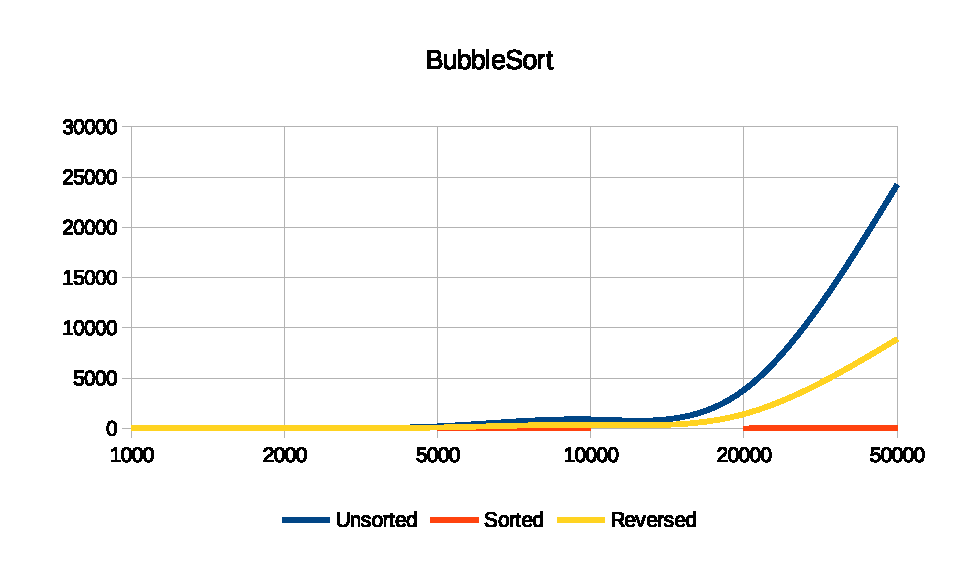
\epsfig{file=BubbleSort2.eps, height=2.5in, width=3.3in}
\caption{Performance for unsorted, sorted and reversed data set.}
\end{figure}

\subsubsection{Average case performance}

In most cases Bubble sort has a time complexity of $O(n^{2})$ and thus making it very inefficient when n grows in size. As we can see from Figure 1, it is very fast in small data sets with less than 10 000 elements, but after about 15 000 elements, the time complexity grows exponentially.
\subsubsection{Best case performance}

For already sorted arrays the time complexity of the algorithm is $O(n)$. This is actually an improved variation of the Bubble sort which  checks if the array is sorted by keeping a flag if there were any swaps during the first iteration through the array. If there were no swaps, the array is sorted and thus with only one iteration we conclude that it is sorted.

\subsubsection{Worst case performance}

Because of the nature of the way the algorithm works, the worst case has the same time complexity as the average case performance.

\subsubsection{Further observations}

From the graph we can see that in the case of a reversed array with more than 15 000 elements, Bubble sort is actually faster than the unsorted array. This is caused by the processor's branch prediction technology which causes the algorithm to be more efficient with a reversed array.

\subsection{InsertionSort}

Insertion sort is one of the most popular algorithms for smaller data sets, because even with arrays of around 50 000 elements, the sorting takes less than 6 000 milliseconds. The algorithm resembles the way that a human sorts things, i.e. a deck of cards. Its simplicity in terms of implementation and stability make it a good choice for relatively small data sets.

\begin{figure}[!htb]
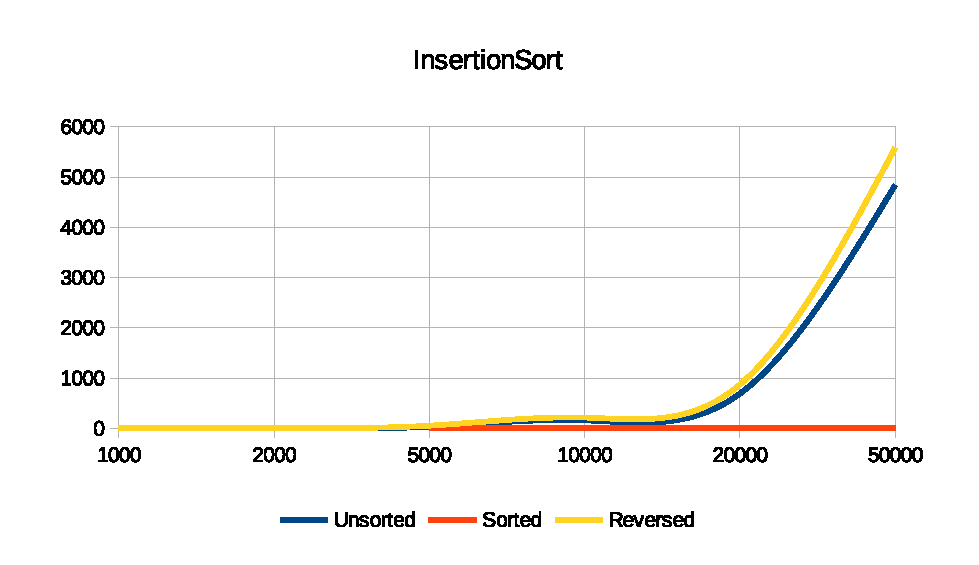
\epsfig{file=InsertionSort.eps, height=2.5in, width=3.3in}
\caption{Performance for unsorted, sorted and reversed data set.}
\end{figure}

\subsubsection{Average case performance}

The average performance of Insertion sort is $O(n^{2})$ with an unsorted array. From Figure 2 we can see that if the size of the array is less than 20 000 the algorithm runs in less than 1 000 milliseconds

\subsubsection{Best case performance}

The best case performance for the algorithm is $O(n)$ comparisons with $O(1)$ swaps. This is in case the array is already sorted or nearly sorted and thus make Insertion sort a good choice to finish sorting after a more complex divide and conquer algorithm is used.

\subsubsection{Worst case performance}

The worst case performance is $O(n^{2})$. When an array is reversed, Insertion sort has a slightly slower performance but still runs within a reasonable time and sorts data sets of sizes between 20 000 and 50 000 in less than 6 000 milliseconds.

\subsection{SelectionSort}

Selection sort is an algorithm which runs relatively slow even with small data sets. With arrays which contain more than 20000 elements the running time grows up to 12 000 milliseconds as we can see from Figure 3.

\begin{figure}[!htb]
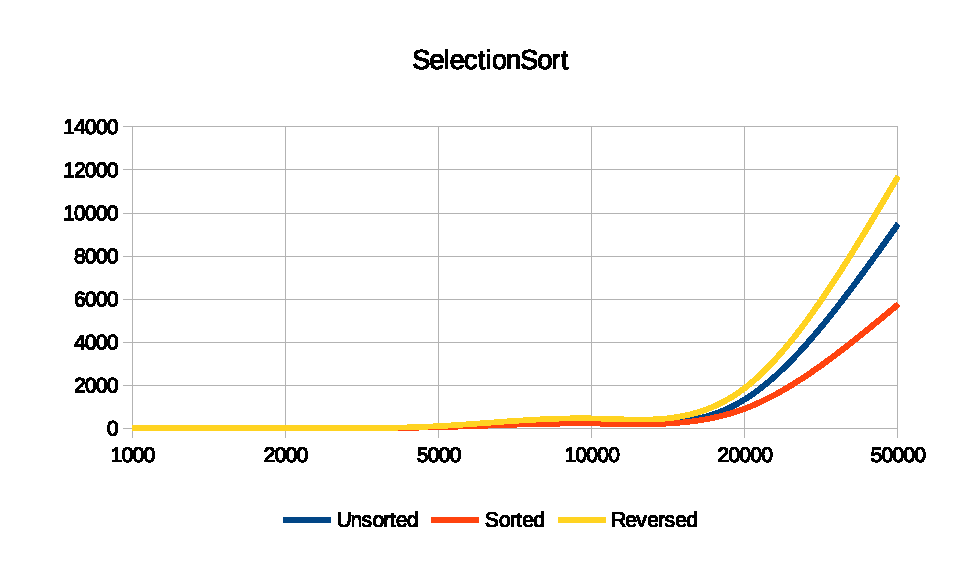
\epsfig{file=SelectionSort.eps, height=2.5in, width=3.3in}
\caption{Performance for unsorted, sorted and reversed data set.}
\end{figure}

\subsubsection{Average case performance}

The average case for Selection sort is $O(n^{2})$. For small data sets up to 15000 elements, the algorithm runs in less than 1 000 milliseconds. 

\subsubsection{Best case performance}

Selection sort's best case performance is $O(n^{2})$ because it iterates multiple times through the array. This is good in cases when the array is nearly sorted and for data sets that are nearly sorted. This causes the running time to be about 6 000 milliseconds which is around two times faster than a reversed array.

\subsubsection{Worst case performance}

The worst case performance for Selection sort is when the array is reversed. It needs to iterate through the entire list to find the lowest value which would always be at the end. This causes a substantial rise in the running time to about 12 000 milliseconds.

\subsection{RadixSort}

Radix sort is an address based algorithm. This means that it does not do comparisons while iterating through an array. It groups up integers with the same significant position and value. This makes the algorithm very fast but at the expense of memory.

\begin{figure}[!htb]
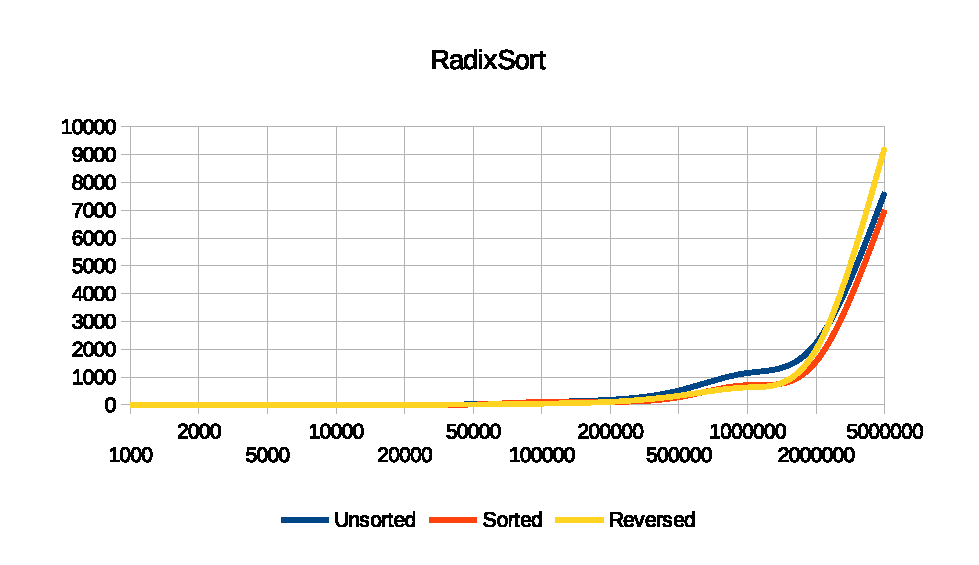
\epsfig{file=RadixSort.eps, height=2.5in, width=3.3in}
\caption{Performance for unsorted, sorted and reversed data set.}
\end{figure}

\subsubsection{Average case performance}

The average time complexity for Radix sort is considered to be $O(d•n)$ for n keys with d or fewer digits. It cannot be assumed that d would be a constant so it is most commonly $logn$. This leads to an overall average time complexity of $O(n•logn)$ for Radix sort. From the graph on Figure 5 we can see that for most arrays with elements up to 5 000 000 it takes about 9 000 milliseconds to run.

\subsubsection{Best case performance}

From Figure 5 we can see that the best performance for Radix sort is with data sets up to 1 500 000 elements. The running time for this size is about 1 000 milliseconds.

\subsubsection{Worst case performance}

For arrays with sizes between 1 500 000 and 5 000 000 elements, the time complexity grows and the run time is at most 9 000 milliseconds for a reversed array. The worst case performance for the algorithm is $O(kN)$ and the worst case in space complexity is $O(k+N)$. The queue data structure used by the algorithm can be very heavy on the memory and this is why the algorithm should be avoided for bigger data sets.

\subsection{ShellSort}

This algorithm can be looked at as an improved version of Insertion sort. A simple addition causes Shell sort to have an average time complexity of $O(n•logn)$. This is caused by an additional variable called the gap. By doing that, values which are smaller can be brought near the beginning of the array even, early on in the process of sorting. However, it is sometimes unstable and if chosen poorly, the gap can lead to bad performance.

\begin{figure}[!htb]
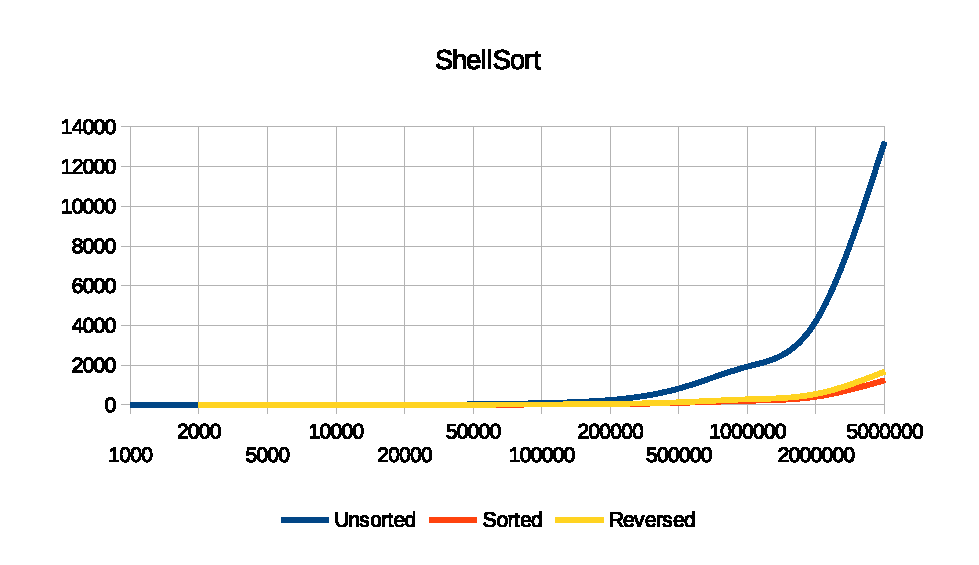
\epsfig{file=ShellSort.eps, height=2.5in, width=3.3in}
\caption{Performance for unsorted, sorted and reversed data set.}
\end{figure}

\subsubsection{Average case performance}

The average case performance is mostly dependant on the gap sequence that is used. For these tests, in each round, the gap is divided by 2.2. From Figure 4 we notice that with this gap, arrays of size up to 1 000 000 are sorted within 2 000 milliseconds for an unsorted array.

\subsubsection{Best case performance}

Shell sort's best case performance can reach up to $O(n•logn)$, mostly on a nearly sorted array. This can be seen from Figure 4 which shows that the running time is within 2 000 milliseconds for data sets as big as 5 000 000 elements.

\subsubsection{Worst case performance}

The worst case time complexity that Shell sort can reach is $O(n^{2})$. This is because the algorithm works very similar to Insertion sort (Section 2.2). If the gap is brought down to 1 in the beginning of the gap sequence, the algorithm works like a basic Insertion sort. This causes the instability of Shell sort.

\subsection{QuickSort}

Quick sort is one of the most robust sorting algorithms. It is used when a stable sort is not needed. A very important part of the performance of Quick sort is the choice of pivot. It can cause big differences in the time complexity. For the tests that are being analyzed in this document, a median value is found and used as the pivot.

\begin{figure}[!htb]
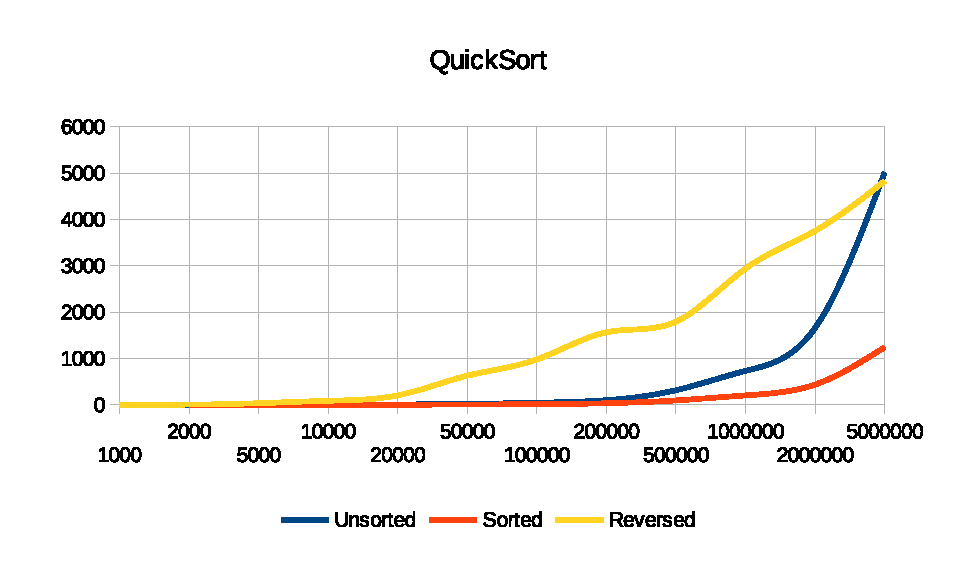
\epsfig{file=QuickSort.eps, height=2.5in, width=3.3in}
\caption{Performance for unsorted, sorted and reversed data set.}
\end{figure}

\subsubsection{Average case performance}

In most cases, Quick sort has a time complexity of $O(n•logn)$. As we can see from Figure 6, arrays with up to 2 000 000 elements are sorted within 2 000 milliseconds.

\subsubsection{Best case performance}

The best case performance of Quick sort is $O(n•logn)$. However this depends on the partitioning method that is used. In this paper, only a simple two-way partitioning is used, but a better variation is a three-way partition. This can lead to a great increase in the best case performance, which can reach $O(n)$. 

\subsubsection{Worst case performance}

The instability of Quick sort can lead to a worst case time complexity of $O(n^{2})$. This happens if the pivot is poorly chosen. Usually a random pivot can be used to lower the chances of $O(n^{2})$ performance.

\subsubsection{Further observations}

With the used method for choosing a pivot - median value, a reversed array is sorted slower even with relatively small data sets. With more than 2 000 elements, the run time grows dramatically compared to the sorted/nearly sorted and unsorted arrays.

\section{Comparisons}

This section will discuss the different sorting algorithms that are explored in this paper and compare them based on their average case time complexity.

\subsection{Comparison of $O(n^{2})$ algorithms}

The algorithms discussed in this section are BubbleSort, InsertionSort and SelectionSort. They have a relatively similar run time.

\begin{figure}[!htb]
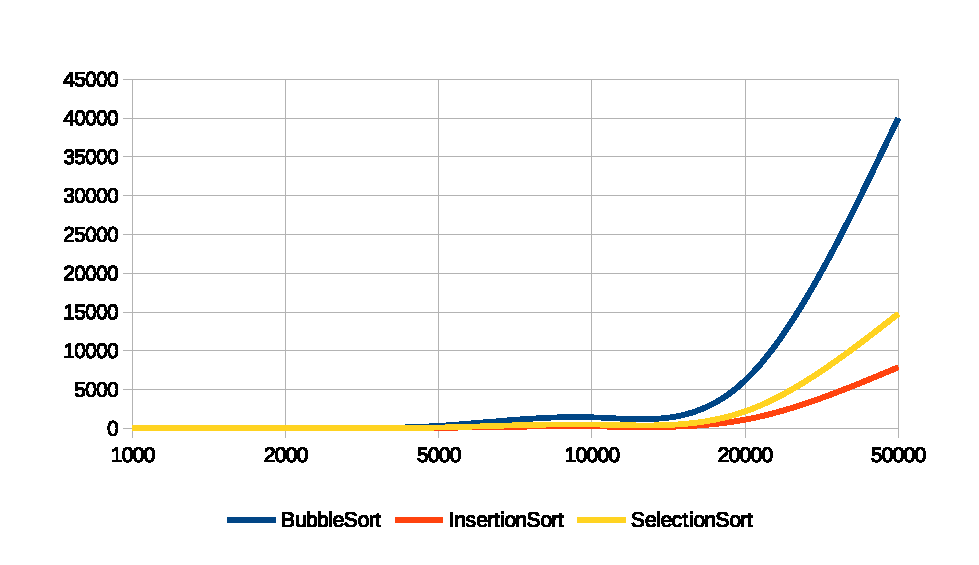
\epsfig{file=n2comparison.eps, height=2.5in, width=3.3in}
\caption{Comparison in run times between the $O(n^{2})$ algorithms.}
\end{figure}

From Figure 7 we can see that for small data sets between 5 000 and 15 000 elements the three algorithms have a similar run time that is within 2 000 milliseconds. However, BubbleSort is slightly slower compared to Insertion and Selection sorts. \\
For data sets larger than 15 000 elements, bigger differences can be observed. BubbleSort's run time grows significantly larger than the other two and reaches up to 40 000 milliseconds run time for an array of 50 000 elements. SelectionSort's run time is much better than BubbleSort and reaches a maximum of 15 000 milliseconds for a data set of 50 000 elements.\\
From these three algorithms, Insertion sort has the best run time with about 7 500 milliseconds run time for the 50 000 elements data set. This makes it the best choice out of these three $O(n^{2})$ algorithms.


\subsection{Comparison of $O(n•logn)$ algorithms}
This section will look into the three discussed $O(n•logn)$ - RadixSort, ShellSort and QuickSort. They all have very high performance and a relatively similar run time.

\begin{figure}[!htb]
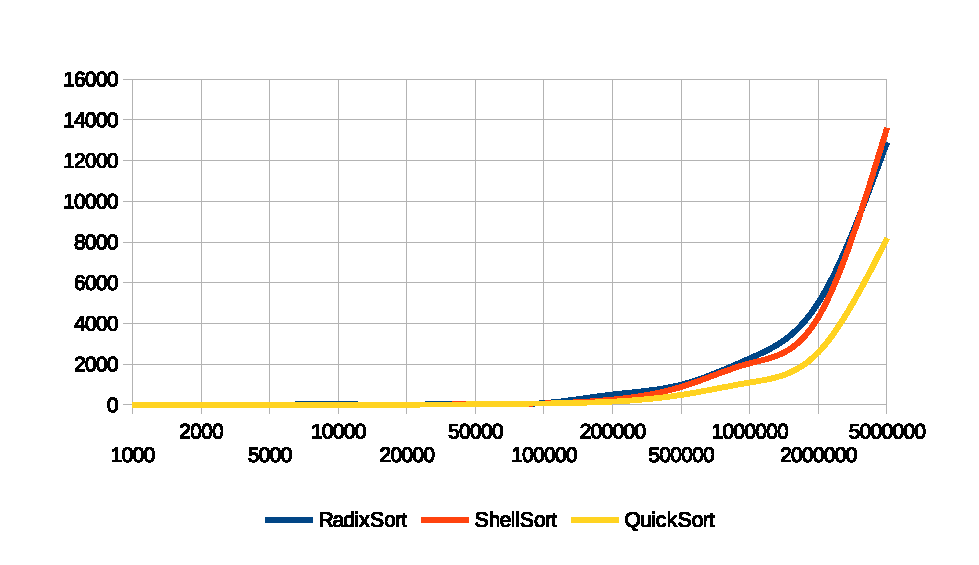
\epsfig{file=nlogncomparison.eps, height=2.5in, width=3.3in}
\caption{Comparison in run times between the $O(n•logn)$ algorithms.}
\end{figure}

From the graph on Figure 8 we can see that for arrays of up to 100 000 elements, the three algorithms perform really well and complete the sorting within a few milliseconds.\\
With data sets between 100 000 and 500 000 elements, there are some more significant differences. RadixSort's run time increases slightly and reaches a maximum of 1 000 milliseconds. However, ShellSort turns out to be a bit faster and QuickSort has the fastest run time within this data set size bracket.\\
When the data set grows between 500 000 and 2 000 000 there are more noticeable differences in run times. RadixSort and ShellSort have a very similar run time which is within 1 000 and around 2 000 milliseconds with data sets that contain less than 1 000 000 elements. QuickSort maintains a maximum of around 1 000 milliseconds run time. For data sets of sizes between 1 000 000 and 2 000 000, ShellSort gains a slight advantage to RadixSort and beats it by a few milliseconds. QuickSort still has the best run time of the three and reaches a maximum of around 2 200 milliseconds for the 2 000 000 elements data set.\\
For arrays of size 2 000 000 to 5 000 000, ShellSort gains advantage over RadixSort and has a slightly better run time. This is because of the fact that smaller values are pushed to the front of the array early on. QuickSort's run time reaches a maximum of 8 000 milliseconds run time for a 5 000 000 elements data set which is significantly faster than the 13 700 milliseconds for ShellSort and 13 000 milliseconds for RadixSort.\\
This concludes that out of the three observed algorithms, QuickSort has the fastest run time and manages quite well with big data sets.

\section{Conclusions}
From the observed algorithms, we can conclude that QuickSort is the best general-purpose sorting algorithm for bigger data sets. However, it is not always good to use QuickSort because of the recursion which is used for the algorithm and may cause memory issues. This is why a combination of two algorithms can be used to form a hybrid one. For example QuickSort can be used to lead the array to a nearly sorted state and after that InsertionSort can be used to finish of the nearly sorted array, because as we previously observed it has a very good performance with smaller data sets.

%ACKNOWLEDGMENTS are optional
\section{Acknowledgments}
Richard Shipman - provided the code for BubbleSort and RadixSort

%
% The following two commands are all you need in the
% initial runs of your .tex file to
% produce the bibliography for the citations in your paper.
\bibliographystyle{abbrv}
\bibliography{sigproc}  % sigproc.bib is the name of the Bibliography in this case
% You must have a proper ".bib" file
%  and remember to run:
% latex bibtex latex latex
% to resolve all references
%
% ACM needs 'a single self-contained file'!
%
%APPENDICES are optional
%\balancecolumns
\balancecolumns
\appendix
%Appendix A
\section{Headings in Appendices}

\subsection{Introduction}
\subsection{Algorithms in detail}
\subsubsection{BubbleSort}
\subsubsection{InsertionSort}
\subsubsection{SelectionSort}
\subsubsection{RadixSort}
\subsubsection{ShellSort}
\subsubsection{QuickSort}
\subsection{Comparisons}
\subsubsection{Comparison of $O(n^{2})$ algorithms}
\subsubsection{Comparison of $O(n•logn)$ algorithms}
\subsection{Conclusions}
\subsection{Acknowledgments}

\subsection{References}
http://www.sorting-algorithms.com/ - Explanations, pseudo-code and visual representations of some sorting algorithms.

http://bigocheatsheet.com/ - Time complexity guide for algorithms.

https://www.khanacademy.org/ - Explanations for some sorting algorithms.
\balancecolumns
% That's all folks!
\end{document}
